%%%%%%%%%%%%%%%%%%%% author.tex %%%%%%%%%%%%%%%%%%%%%%%%%%%%%%%%%%%
%
% sample root file for your "contribution" to a contributed volume
%
% Use this file as a template for your own input.
%
%%%%%%%%%%%%%%%% Springer %%%%%%%%%%%%%%%%%%%%%%%%%%%%%%%%%%


% RECOMMENDED %%%%%%%%%%%%%%%%%%%%%%%%%%%%%%%%%%%%%%%%%%%%%%%%%%%
\documentclass[graybox]{svmult}

% choose options for [] as required from the list
% in the Reference Guide

\usepackage{type1cm}        % activate if the above 3 fonts are
                            % not available on your system
%
\usepackage{makeidx}         % allows index generation
\usepackage{graphicx}        % standard LaTeX graphics tool
                             % when including figure files
\usepackage{multicol}        % used for the two-column index
\usepackage[bottom]{footmisc}% places footnotes at page bottom


\usepackage{newtxtext}       % 
\usepackage{newtxmath}       % selects Times Roman as basic font
\usepackage[utf8]{inputenc}
\DeclareUnicodeCharacter{2082}{$_2$}
\DeclareUnicodeCharacter{00B2}{\textsuperscript{2}}

% see the list of further useful packages
% in the Reference Guide

\makeindex             % used for the subject index
                       % please use the style svind.ist with
                       % your makeindex program

%%%%%%%%%%%%%%%%%%%%%%%%%%%%%%%%%%%%%%%%%%%%%%%%%%%%%%%%%%%%%%%%%%%%%%%%%%%%%%%%%%%%%%%%%

\begin{document}

\title*{Ecosystem-Based Spatial Validation of Machine Learning
Models for Global Plant Transpiration Prediction
}
% Use \titlerunning{Short Title} for an abbreviated version of
% your contribution title if the original one is too long
\author{Roberto Palacios}
% Use \authorrunning{Short Title} for an abbreviated version of
% your contribution title if the original one is too long
\institute{Roberto Palacios \at California State University, 100 Campus Ctr, Seaside, CA 93955, \email{rpalacios@csumb.edu}
\and Name of Second Author \at Name, Address of Institute \email{name@email.address}}
%
% Use the package "url.sty" to avoid
% problems with special characters
% used in your e-mail or web address
%
\maketitle


\abstract{
Sap flux is a widely used and reliable method for tracking plant-scale transpiration. However, collecting sap flux data is relatively expensive compared to measuring environmental variables that influence transpiration, such as vapor pressure deficit or radiation. While prior research has demonstrated the potential of machine learning (ML) to predict sap flux at individual sites, it remains unclear whether such models can generalize across ecologically diverse locations.
To address this gap, we present an end-to-end workflow for defining ecologically meaningful site clusters within the SAPFLUXNET database and training separate XGBoost models per cluster using over 23 years of data from 87 sites across 5 biomes. Generalization performance is assessed using leave-one-out cross-validation (LOOCV) that withholds entire sites. 
Predictive accuracy varied widely between held-out sites, resulting in a low average test $R^2$ of $-4.07$ and RMSE of 5.46 even within the best-performing cluster. These results indicate that model performance observed in previous studies, where partial site data was available for training, does not transfer to settings with complete site-level separation. We conclude that ecosystem-specific modeling requires either site calibration, richer feature sets, or methods explicitly addressing domain shift to achieve cross-site generalization.}

\section{Introduction}
\label{sec:1}
Transpiration is a stomatal process whereby plants regulate water loss and CO₂ uptake with the surrounding atmosphere \cite{mott_stomatal_2010}. At scale, this process influences land-atmosphere exchange of terrestrial water and holds significant influence over carbon cycles \cite{poyatos_global_2021}. Direct measurement of transpiration is challenging because it is a diffuse, continuous process that occurs at microscopic scales and is influenced by a range of environmental factors, such as wind and solar exposure. Sap flux measurements provide close estimates of transpiration at high-frequency intervals, but require field campaigns that are logistically demanding relative to the effort required to gather data of environmental drivers \cite{poyatos_global_2021}. To improve the spatial coverage and interpretability of sap flux measurements, researchers often incorporate complementary data, including remotely sensed environmental variables \cite{ellsaser_predicting_2020}.

These ensemble datasets have proved instrumental in training machine learning (ML) models that can predict sap flux accuracy at the site level \cite{ellsaser_predicting_2020, kabala_reconstruction_2025}, but whether the same practices can be used to generalize across sites is yet to be seen. The challenge in cross-site generalization stems from variations vegetation composition and environmental drivers across biomes \cite{poyatos_global_2021, peel_updated_2007}. Inconsistency in these factors and their interactions across sites result in domain shift, where the statistical properties of the training data differs from that of the test data \cite{moreno-torres_unifying_2012, quinonero-candela_dataset_2009}. These changes result in shifting relationships between inputs and sap flux which in turn increase the risk overfitting and reduce prediction reliability \cite{liu_soil_2020, zheng_divergent_2023, tyree_hydraulic_2003}. To combat inflated estimates of sap flux predictions, spatial validation strategies assess model transferability while avoiding spatial and temporal data leakage \cite{roberts_crossvalidation_2017, trachsel_telford_2016}.

To investigate cross-site generalization at scale, we used data from 87 sites with 23 years of records across 5 biomes from the SAPFLUXNET database \cite{poyatos_global_2021}. For this purpose, we applied an end-to-end workflow that first groups sites into ecologically meaningful clusters and then trains separate XGBoost models for each cluster \cite{chen_xgboost_2016}. Clusters are defined to be ecologically meaningful using long-term climate normals, biome descriptors, and geolocation to reflect environmental similarity rather than site identity. We evaluate model performance under strict spatial validation, including protocols that withhold entire sites \cite{roberts_crossvalidation_2017}. This procedure grants us insight into which predictions fail to transfer across ecological contexts.

As part of the process, we performed our validation within sets of clusters designed to increase ecological homogeneity. We evaluated model performance using leave-one-site-out (LOSO) within clusters, retraining from scratch each fold to avoid leakage. Under this protocol, predictive accuracy varies widely across held-out sites, leading to low average test performance  (mean test $R^2=-4.07$, RMSE=5.46). Our finding indicate that results reported under within-site or partially pooled conditions fail to generalize effectively to novel sites, underscoring the need for domain-aware modeling strategies \cite{moreno-torres_unifying_2012, quinonero-candela_dataset_2009}.

\section{Related Work and Background}
\label{sec:2}

The work presented in this paper builds on prior research in sap flux measurement logistics; the environmental and physiological drivers of transpiration; machine learning methods for sap flux prediction; clustering techniques for model partitioning; and spatial validation strategies.

\subsection{Sap flux datasets and measurement context}
SAPFLUXNET is the first global compilation of quality-controlled whole-plant transpiration time series data derived from sap flow measurements \cite{poyatos_global_2021}. Sap flux provides direct, plant-scale estimates of transpiration at regular, high frequencies. However, gathering sap flux measurements require specialized sensors, infrastructure, and sustained field effort, resulting in field campaigns with higher opportunity costs relative to routine meteorological data streams \cite{poyatos_global_2021}. Thus exists the push for methods which augment existing or missing data with more readily available complementary drivers and proxies (e.g. photosynthetic photon flux density, vapor pressure deficit, temperature) \cite{ge_dynamics_2011}.

\subsection{Environmental controls and plant hydraulics}
Water loss (e.g. transpiration) and CO$_2$ assimilation in plants is regulated by the stomatal activity \cite{mott_stomatal_2010}. As such, stomatal activity varies not only across sites but plants as they each experience unique interactions among moisture, atmospheric conditions, thermal stress and light exposure \cite{liu_soil_2020, zheng_divergent_2023}. Furthermore, responses are constrained by plant hydraulics and short-term acclimation to antecedent environmental conditions, thereby requiring interpretations of transpiration readings to account for these confounding factors. \cite{tyree_hydraulic_2003, poirier-pocovi_sensitivity_2020, anav_sensitivity_2018, jiang_optimalitybased_2020, stocker_p-model_2020}. One approach is to work within climate regions that aid in partitioning data into areas of strong heterogeneity in drivers for improved modeling and analysis \cite{peel_updated_2007}.

\subsection{Machine learning for transpiration and sap flux}
Sap flux and stomatal conductance have been successfully predicted with high accuracy at individual sites using previous readings coupled with complementary meteorological and/or remote-sensing inputs \cite{ellsaser_predicting_2020, kabala_reconstruction_2025}. These works rely on randomly or temporally blocked, within-site validation where previous data informs future predictions. Given the complex nature between sap flux and site-specific drivers, the transferability of such models across sites and biomes remains a question that motivates this work.

\subsection{Clustering, modeling, and interpretation}
Removing site identity from training data is key in inducing cross-site generalization as it helps the model learn patterns not specific to any given site. Ecologically focused clusters based on climate normals can help to preserve driver heterogeneity within similar sites \cite{peel_updated_2007}. Gradient-boosted trees (XGBoost) capture the kind of non-linear relationships common in SAPFLUXNET's tabular data \cite{chen_xgboost_2016}. To further improve performance, hyperparameter optimization can be performed with widely available frameworks which provide reproducible results \cite{akiba_optuna_2019}.

\subsection{Generalization, dataset shift, and spatial validation}
Applying trained models to previously unknown sites where the domain differs exposes conditional responses in covariates, and target distributions \cite{moreno-torres_unifying_2012, quinonero-candela_dataset_2009}. Spatially blocked evaluation prevents spatial and temporal leakage within a dataset, thereby producing generalization results that are truer to real conditions \cite{roberts_crossvalidation_2017}. Related work in paleoecology likewise emphasizes unbiased estimation under spatial structure and careful blocking strategies \cite{trachsel_telford_2016}. Together, these insights motivate our use of ecologically informed clustering and strict site-level holdout to assess transferability.

\section{Data and Methodologies}
\label{sec:3}
This study uses publicly available, harmonized sap flux data from SAPFLUXNET and evaluates cross-site generalization via ecologically informed clustering and per-cluster supervised models. We do not collect new data; our contributions are in preprocessing, clustering, model training, and spatial validation design. Figure~\ref{fig:pipeline} summarizes the workflow.

\begin{figure}[p]
  \centering
  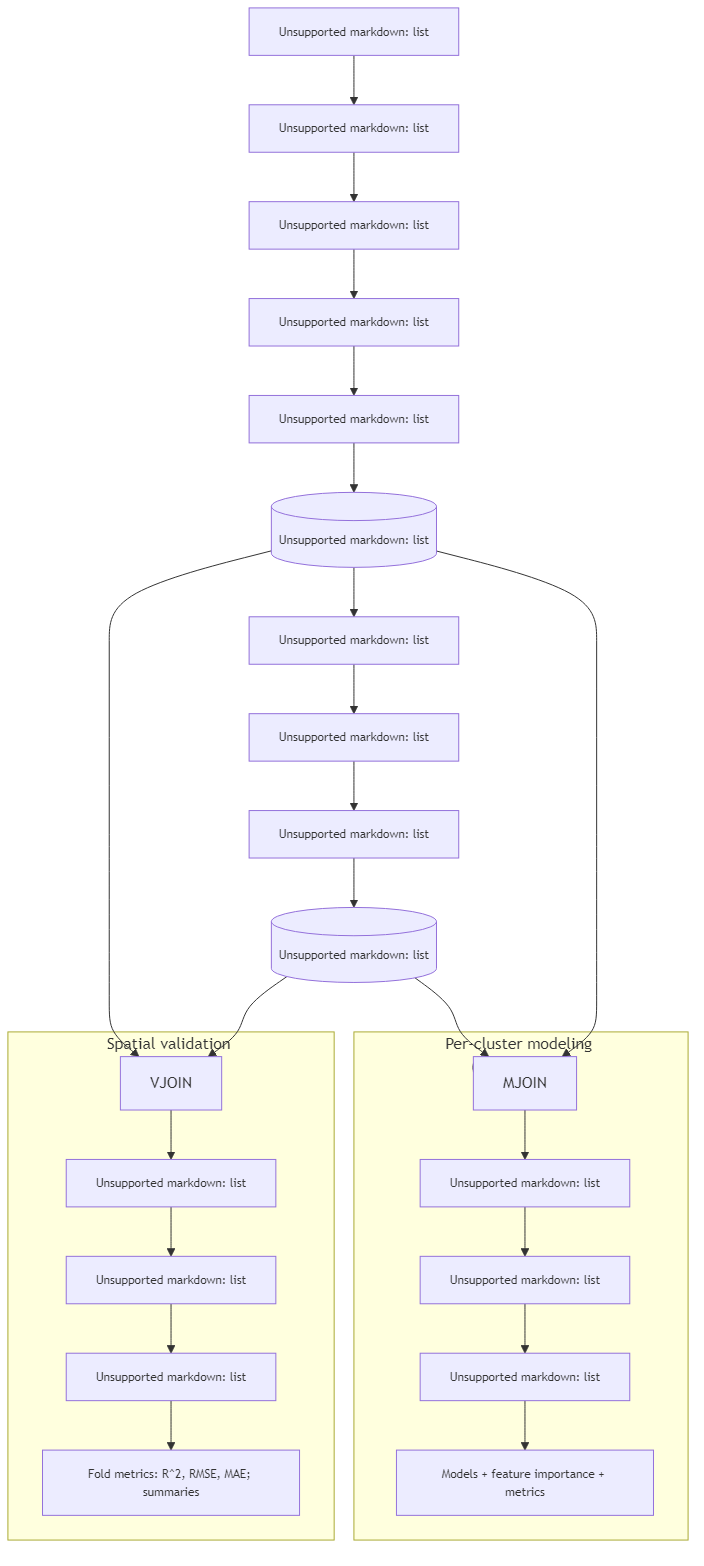
\includegraphics[width=\textwidth,height=0.9\textheight,keepaspectratio]{figures/pipeline_flowchart.png}
  \caption{End-to-end workflow with optional HPO before training and pre-validation; LOSO retrains per fold.}
  \label{fig:pipeline}
\end{figure}
\clearpage

\subsection{Data source and availability}
\label{subsec:data_source}
\textbf{Dataset.} SAPFLUXNET v0.1.5 provides quality-controlled, whole-plant sap flux time-series, associated meteorological drivers, and rich site/stand metadata \cite{poyatos_global_2021}. \\
\textbf{Scope.} We analyze a subset covering 87 sites over 23 years spanning 5 biomes, as represented in our working dataset. \\
\textbf{Variables.} The target is sap flow; drivers include shortwave radiation(SW), vapor pressure deficit(VPD), air temperature(TA), precipitation, relative humidity(RH), and selected metadata-derived features. \\
\textbf{Access.} SAPFLUXNET is publicly available (see \cite{poyatos_global_2021}); no new measurements were collected in this work.

\subsection{Preprocessing and feature construction}
\label{subsec:preprocess}
\textbf{Harmonization.} We rely on SAPFLUXNET harmonization and remove rows missing our target. \\
\textbf{Engineered features (overview).} Temporal lags and rolling statistics; diurnal/seasonal encodings; interaction terms among meteorological drivers; and selected metadata-derived features. Feature policy explicitly avoids site-identity leakage. \\
\textbf{Exclusion policy.} Identity/proxy columns (e.g., site identifiers), timestamps, and feature-quality columns are excluded from modeling inputs. \\
\textbf{Missing values.} Non-numeric columns are coerced to numeric; remaining missing values in feature columns are imputed with zeros consistent with the training path (i.e., \texttt{fillna(0)} after coercion). \\
\textbf{Dimensionality reduction.} None is applied for preprocessing; any PCA usage is limited to visualization, not clustering or modeling.

\paragraph{Inclusion/exclusion.}
We retain rows with valid target (\texttt{sap\_flow}) and drop rows with missing target. Modeling inputs exclude identity/proxy columns (e.g., \texttt{site}, \texttt{plant\_id}), timestamps (\texttt{TIMESTAMP}, \texttt{solar\_TIMESTAMP}), unnamed indices (\texttt{Unnamed: 0}), and columns with suffixes \texttt{\_flags} or \texttt{\_md}. Feature columns are coerced to numeric; remaining missing feature values are imputed with zeros (\texttt{fillna(0)}).

\subsection{Ecologically informed clustering}
\label{subsec:clustering}
\textbf{Goal.} Group sites by environmental/ecological similarity rather than identity. \\
\textbf{Clustering features.} Long-term climate normals and biome descriptors, optionally combined with geolocation to reflect macro-environmental regimes \cite{peel_updated_2007}. \\
\textbf{Standardization.} Features are standardized to zero mean and unit variance prior to clustering. \\
\textbf{Strategy selection.} Common algorithms (e.g., KMeans, Agglomerative, Gaussian Mixture) are considered; the number of clusters and strategy are selected based on internal diagnostics (e.g., silhouette) and cluster balance. Final site-to-cluster assignments drive downstream training and evaluation.

\subsection{Modeling (per cluster)}
\label{subsec:modeling}
\textbf{Learner.} Gradient-boosted decision trees (XGBoost) capture nonlinear interactions and scale efficiently for tabular ecohydrological data \cite{chen_xgboost_2016}. \\
\textbf{Hardware.} GPU acceleration (\texttt{gpu\_hist}) is used when available; CPU (\texttt{hist}) is the fallback. \\
\textbf{Training.} One regressor per cluster trained on sites in that cluster only. Rows with missing target are dropped; feature coercion and NaN handling follow preprocessing above. \\
\textbf{Metrics.} Test $R^2$, RMSE, and MAE are reported for each fold and summarized per cluster.

\paragraph{Hyperparameters.}
We use sensible defaults for XGBoost; where tuning is performed, we use Optuna with leakage-aware folds and bounded search spaces for reproducibility and efficiency \cite{akiba_optuna_2019}. Any tuned configuration is re-trained from scratch on training folds; the held-out site remains unseen until testing.

\begin{table}[ht]
  \centering
\caption{XGBoost hyperparameters used (GPU primary; CPU legacy)}
\begin{tabular}{lcc}
\hline
Parameter & GPU & CPU (legacy) \\
\hline
tree\_method & gpu\_hist & hist \\
max\_depth & 8 & 8/7/6 (adaptive) \\
learning\_rate & 0.10 & 0.10 \\
subsample & 0.8 & 0.8 \\
colsample\_bytree & 0.8 & 0.8 \\
n\_estimators & 300 & 100 (default) \\
max\_bin & -- & 512/256/128 (adaptive) \\
random\_state & \multicolumn{2}{c}{42} \\
\hline
\end{tabular}
\end{table}

\subsection{Spatial validation protocol}
\label{subsec:validation}
\textbf{Within-cluster LOSO.} For each fold, one site is held out for testing; models are retrained from scratch on the remaining sites in the same cluster, preventing spatial/temporal leakage and mimicking deployment to unseen sites \cite{roberts_crossvalidation_2017}. \\
\textbf{Aggregation.} We report fold-level metrics, cluster summaries, and cross-cluster summaries; negative $R^2$ values are retained to reflect true generalization difficulty. \\
\textbf{Dataset shift context.} Cross-site LOSO directly evaluates performance under conditional shifts typical across sites \cite{moreno-torres_unifying_2012, quinonero-candela_dataset_2009}.

\paragraph{Metrics.}
We report test $R^2$, RMSE, and MAE per fold and summarize by cluster. Definitions:
\[
R^2 = 1 - \frac{\sum_{i=1}^{n} (y_i - \hat{y}_i)^2}{\sum_{i=1}^{n} (y_i - \bar{y})^2}
\]
\[
\mathrm{RMSE} = \sqrt{\frac{1}{n}\sum_{i=1}^{n} (y_i - \hat{y}_i)^2}
\]
\[
\mathrm{MAE} = \frac{1}{n}\sum_{i=1}^{n} \lvert y_i - \hat{y}_i \rvert
\]
Negative $R^2$ values are retained to reflect true generalization difficulty.

\subsection{Implementation and reproducibility}
\label{subsec:repro}
\textbf{Stack.} Python; \texttt{xgboost} for learning; \texttt{pandas}/\texttt{numpy} for data handling; standard preprocessing utilities. \\
\textbf{Reproducibility.} We fix random seeds where applicable; record cluster assignments, model artifacts, and evaluation outputs; and avoid reusing fitted models across folds to prevent leakage.

\subsection{Data availability}
SAPFLUXNET v0.1.5 is publicly available via Zenodo (see \cite{poyatos_global_2021}). We used only publicly released data and did not collect new measurements.

\section{Results}
\label{sec:4}
Generalization performance is measured through spatial leave-one-site-out (LOSO) validation within clusters, which is then compared to baseline performance produced by an 80/20 test/train split as our stand-in for an in-sample fit. Test results report $R^2$ (including negative values), RMSE, and MAE for fold-level, cluster-level, and overall summaries.

\subsection{Cluster split training performance}
Training 80/20 splits within heterogeneous clusters produce moderate fits ($R^2 > 75\%$) across all tested clustering schemes and feature sets. Aggregate training summaries show non-trivial fit in-sample, yet these results do not translate into LOSO performance. Per-cluster training metrics and an overall summary are saved alongside models; we reference these for descriptive completeness but do not use them to infer generalization.

\subsection{Spatial validation (LOSO within clusters)}
LOSO results show a deep degree of variance among held-out sites within the same cluster with many results showing negative test $R^2$. For the best-performing cluster, mean test $R^2\approx -4.07$ and RMSE $\approx 5.46$—values far below the established baseline of the cluster split results. Meanwhile, cluster-level summaries detail inconsistent performance with large standard deviations for $R^2$ and RMSE values across clusters despite the coherent ecological nature of the clusters. To detail the depth of error in these trials, we retained negative values as truncating at 0 would misinform the challenge of the situation. These performance gaps indicate that complete site separation poses a hurdle to cross-site generalization. The distribution of scores shows that some sites can be predicted with modest success, but many sites per cluster show sizable errors due to pronounced domain shift.

\subsection{Hyperparameter optimization}
Hyperparameter tuning performed with Optuna yields cluster-specific parameter sets which, when used to retrain folds from scratch, produced small changes in mean fold metrics. Overall, variability across sites and parameter tuning did not ease the effects of domain shift or change the overall conclusion of the project. As such, the inclusion of hyperparameter optimization here is merely as an optional set that helps ensure robustness of our results.

\subsection{Feature importance and patterns}
Feature importance varies by cluster, indicating that the response of each grouping is governed by shifting factors. Vapor pressure deficit, shortwave radiation, air temperature, and diurnal/seasonal encodings are consistently influential but rank differently across clusters. Lagged and rolling features also rank highly, indicating sensitivity to short-term antecedent states.

\subsection{Failure modes and uncertainty}
Errors are largest at sites where the test data differs greatly from training data in the same cluster due to domain shift. Prediction errors increase as extreme atmospheric demands drive transpiration and widen the gap between the train and test conditions. These patterns align with domain shift as the primary limitation to generalization, rather than model capacity.

\subsection{Computational notes}
While XGBoost is well suited for CPU training, GPU acceleration exponentially reduces training/validation time per fold; a significant material improvement as all models are retrained per fold during LOSO.

\subsection{Summary of findings}
Non-trivial performance during within-cluster training does not anticipate generalization success. LOSO validation shows high predictive variance across held-out sites, with low or negative mean test $R^2$ at the cluster level and a high spread of RMSE values. Hyperparameter optimization alters parameters but does not resolve cross-site domain shifts. Feature-importance patterns indicate that richer, site‑calibrated feature sets are necessary for transferable performance.
\section{Conclusion}
\label{sec:5}
We evaluated cross-site transferability of sap flux prediction using ecologically informed clustering and per-cluster XGBoost models. Under strict within-cluster LOSO validation, predictive accuracy varies widely across held-out sites, with low or negative mean test $R^2$ at the cluster level (e.g., $\approx -4.07$ in the best-performing cluster) and large RMSE dispersion. In contrast, within-cluster 80/20 training splits yield moderate in-sample fits, which do not anticipate spatial generalization. Hyperparameter optimization changes model settings but does not resolve cross-site regime mismatch. Feature-importance patterns differ by cluster, indicating shifting controls across regimes. Together, these findings identify domain shift—not limited model capacity—as the primary barrier to transferability and motivate domain-aware solutions.

\subsection{Applications} %
For within-site gap-filling and short-term forecasting, the models provide practical value when trained and validated in-sample. For cross-site deployment, however, reliable performance requires either site calibration, domain-adaptation strategies, or richer, site-calibrated feature sets (e.g., trait, soil, stand structure, and protocol metadata). We recommend spatially blocked evaluation (LOSO) during development and reporting negative $R^2$ where appropriate to avoid optimistic assessments. In operational settings, monitoring covariate shift and flagging out-of-distribution conditions can guide confidence and model fallback behavior.

\subsection{Concerns and Next Steps} %
This study is limited by coverage biases in SAPFLUXNET, heterogeneous measurement protocols, a restricted feature set, and focus on a single learner family. Future work should (i) incorporate domain adaptation and hierarchical approaches to handle regime mismatch; (ii) expand feature sets with site-calibrated and remote-sensing covariates; (iii) standardize and leverage protocol metadata; (iv) quantify and communicate uncertainty; and (v) benchmark additional learners and representation-learning methods. Ultimately, transferable sap flux prediction will require models that explicitly account for cross-site distributional differences while preserving ecological interpretability.
%

\begin{acknowledgement}
If you want to include acknowledgments of assistance and the like at the end of an individual chapter please use the \verb|acknowledgement| environment -- it will automatically be rendered in line with the preferred layout.
\end{acknowledgement}



% Bibliography
\bibliography{sapfluxworks}
\bibliographystyle{plain}

\end{document}
